Nous étudions la viabilité des RK-ImEx sur l'équation de Nagumo. Pour cela nous étudions sa stabilité.
Dans un premier temps, une étude générale de la stabilité de des RK-ImEx est menée.
Dans un second temps, l'étude se centre sur l'application à l'équation de Nagumo.

\subsubsection{Étude de stabilité générale des RK-ImEx}
    Lorsque l'on use d'une méthode ImEx, les deux (ou plus) opérateurs sont découplés, c'est bien là l'intérêt.
    Cependant cela complique légèrement l'analyse usuelle de stabilisé. En effet la fonction de stabilité attend alors deux variables, %AFAIRE -> ajouter les renvois vers la partie introduction à l'étude de stabilité etc...
    le coefficient spectral associé à l'opérateur traité explicitement et le coefficient spectral associé à l'opérateur traité implicitement.
    Ainsi, pour chaque couple de valeur propre, la fonction de stabilité prend une valeur différente et comme les coefficients spectraux sont complexes, 
    on ne peut plus visualiser d'un simple coup d'œil le domaine de stabilité (comme en ... AFAIRE), puisque celui-ci est de dimension quatre
    \footnote{En effet la fonction de stabilité $R \mathbb C \times \mathbb C \rightarrow \mathbb R$ et $\dim  \mathbb C \times \mathbb C=4$.}.
    \paragraph{Calcul des fonction d'amplification }
    Afin d'étudier la stabilité linéaire des méthodes, les fonctions d'amplifications ont été numériquement.
    %AFAIRE ---> faire les calculs analytiques ... :)


\subsubsection{Étude de stabilité appliquée à l'équation de Nagumo}
    Nous allons particulariser la démarche suivante en la centrant sur l'équation de Nagumo. Cela vas nous permettre de comprendre 
    comme se comportent les méthodes ImEx sur ce problème particulier.
    \paragraph{Valeurs propres mises en jeu}
        Comme expliqué en \ref{par:analyser_operateurs_nagumo} l'équation présente deux opérateurs : 
        \begin{itemize}
            \item[$\diamond$] La diffusion dont le spectre d'étend de $\frac{-1}{L^2}$ à $\frac{-1}{\Delta x^2}$ (où $L$ est la taille du domaine discrétisé).
            \item[$\diamond$] La réaction dont le spectre balaie continûment $-k$ jusqu'à $2k$
        \end{itemize}
        Pour restreindre l'analyse de stabilité il faut donc tracer le diagramme de stabilité des méthodes étudiées en prenant $Z_I \in \mathbb{R}^-$ 
        et $Z_E \in [-k;2k] \subset \mathbb{R}$ ce qui nous donne un espace à deux dimensions. Il faut ensuite placer des couples $(Z_E,Z_I)$ correspondant.
        Lorsque l'on réalise se travaille nous trouvons les diagrammes suivant: 
    \paragraph{Résultats}
    \begin{figure}[htbp]
        \centering
        
        \begin{subfigure}{\textwidth}
            \centering
            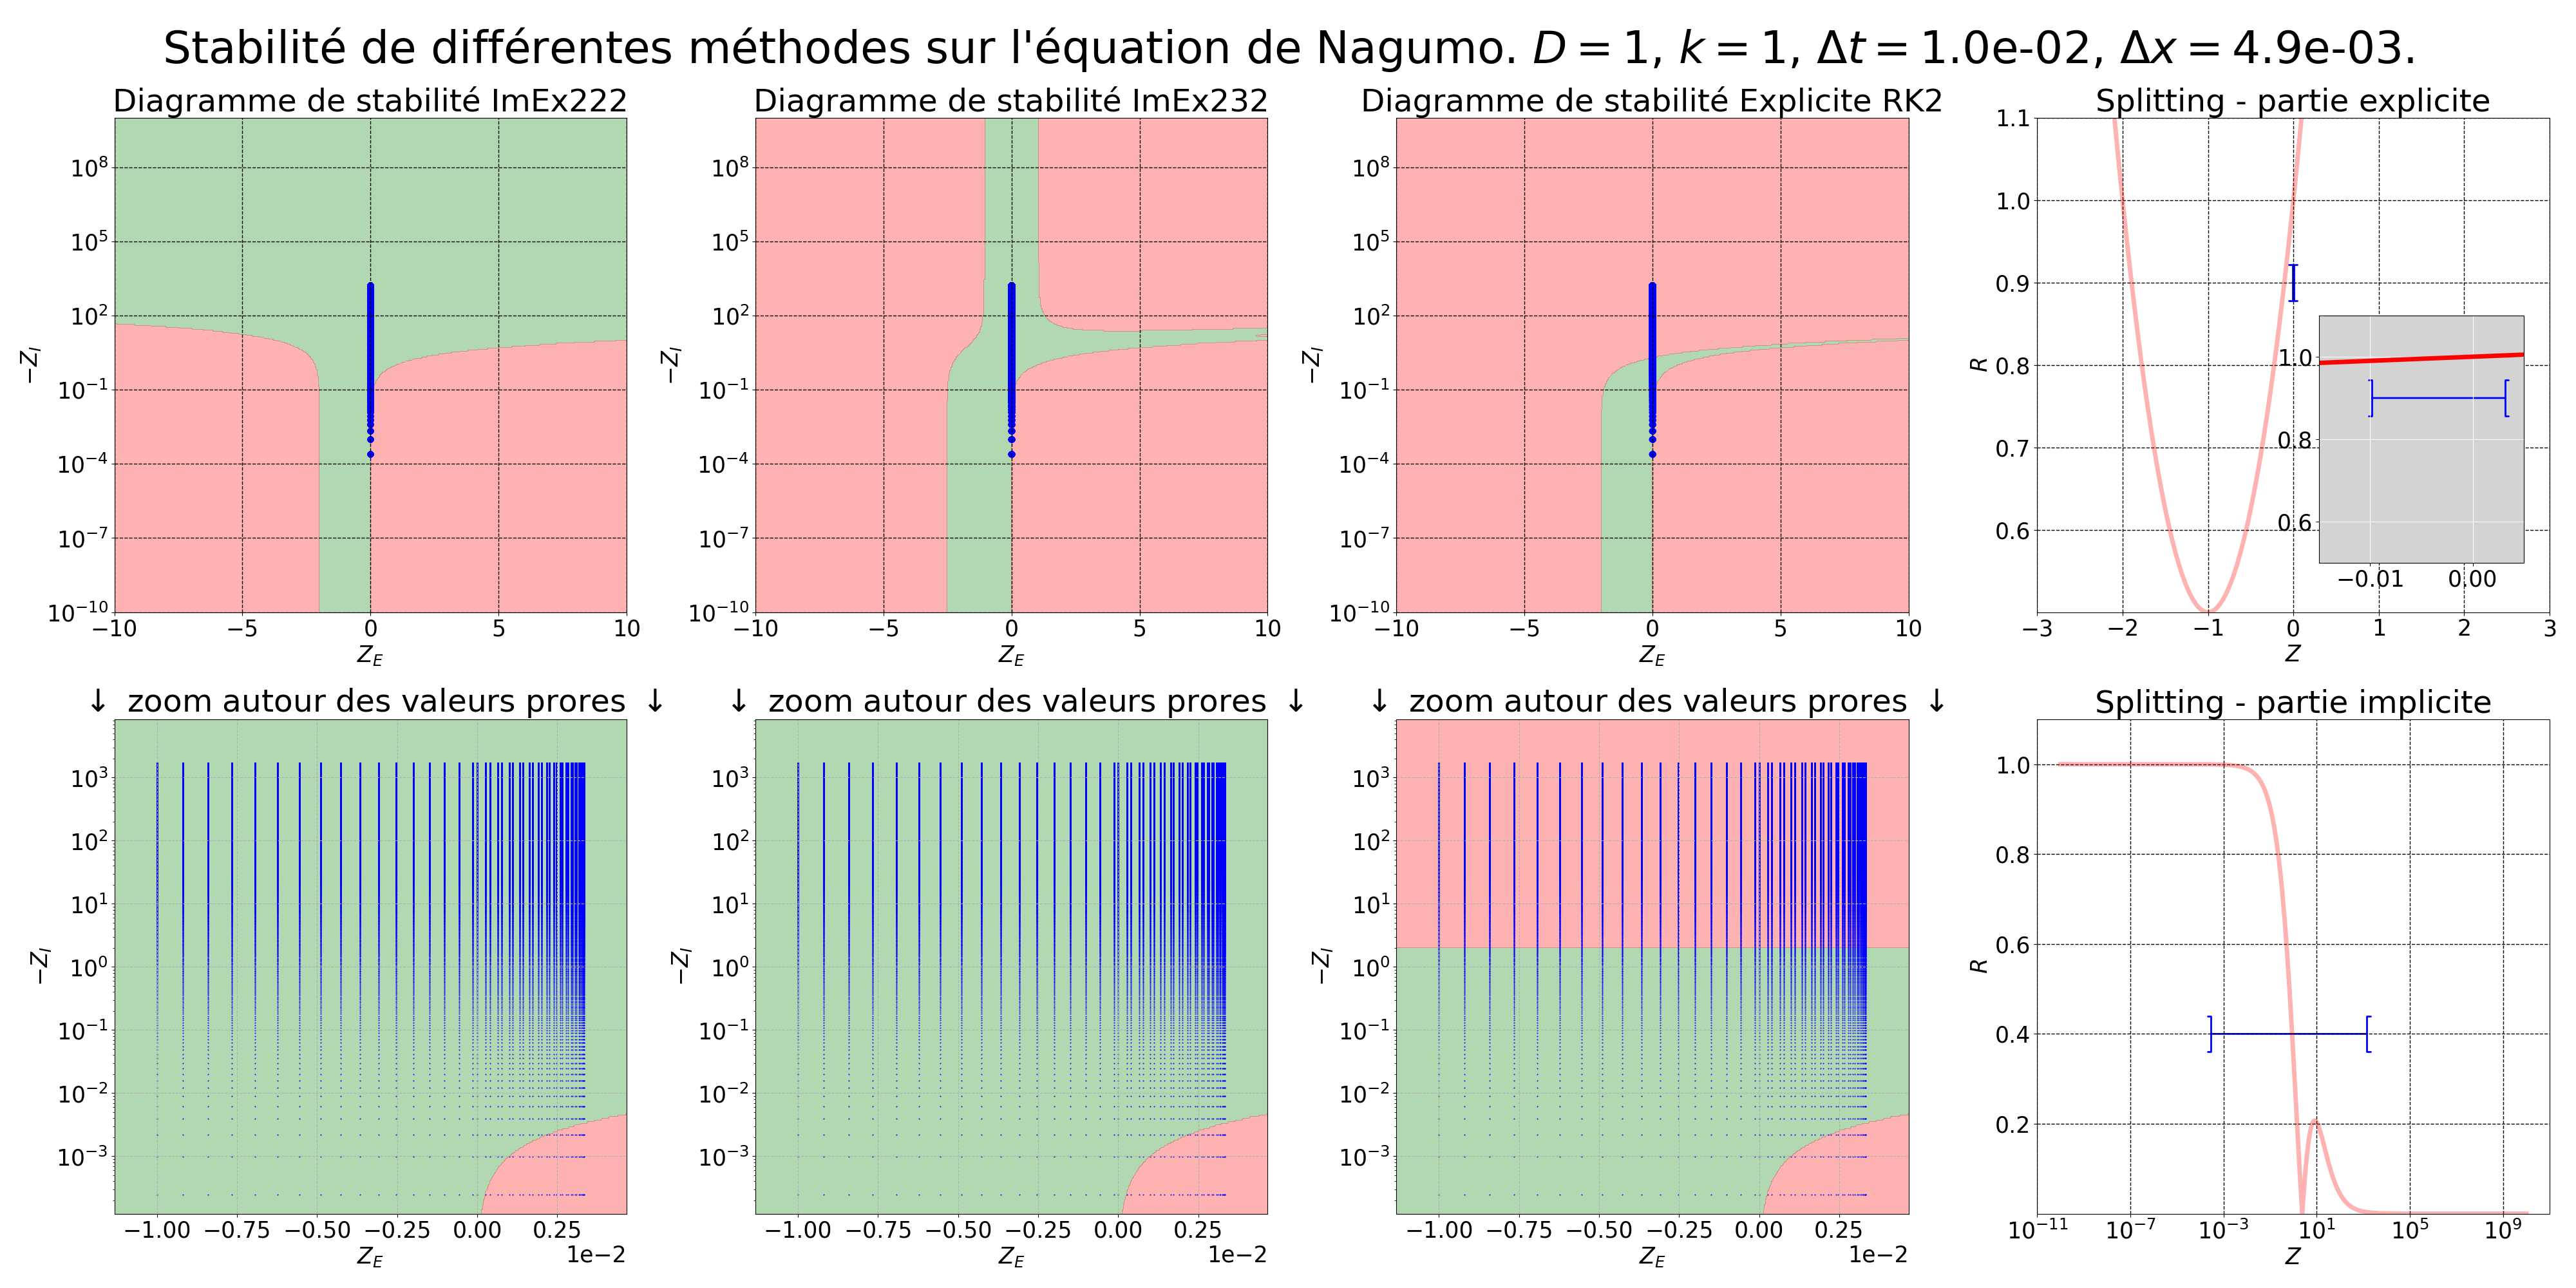
\includegraphics[width=0.8\textwidth]{media/4_travail/2_nagumo/stabilite/STABILITE_D1_k1_dt1.0e-02_dx4.9e-03.png}
            \caption{Cas standard\\D=1, k=1, dt=1.0e-03, dx=2.4e-03}
            \label{fig:stabilite_nagumo_a}
        \end{subfigure}
        
        \vspace{0.5cm} % Espacement entre les sous-figures
        
        \begin{subfigure}{\textwidth}
            \centering
            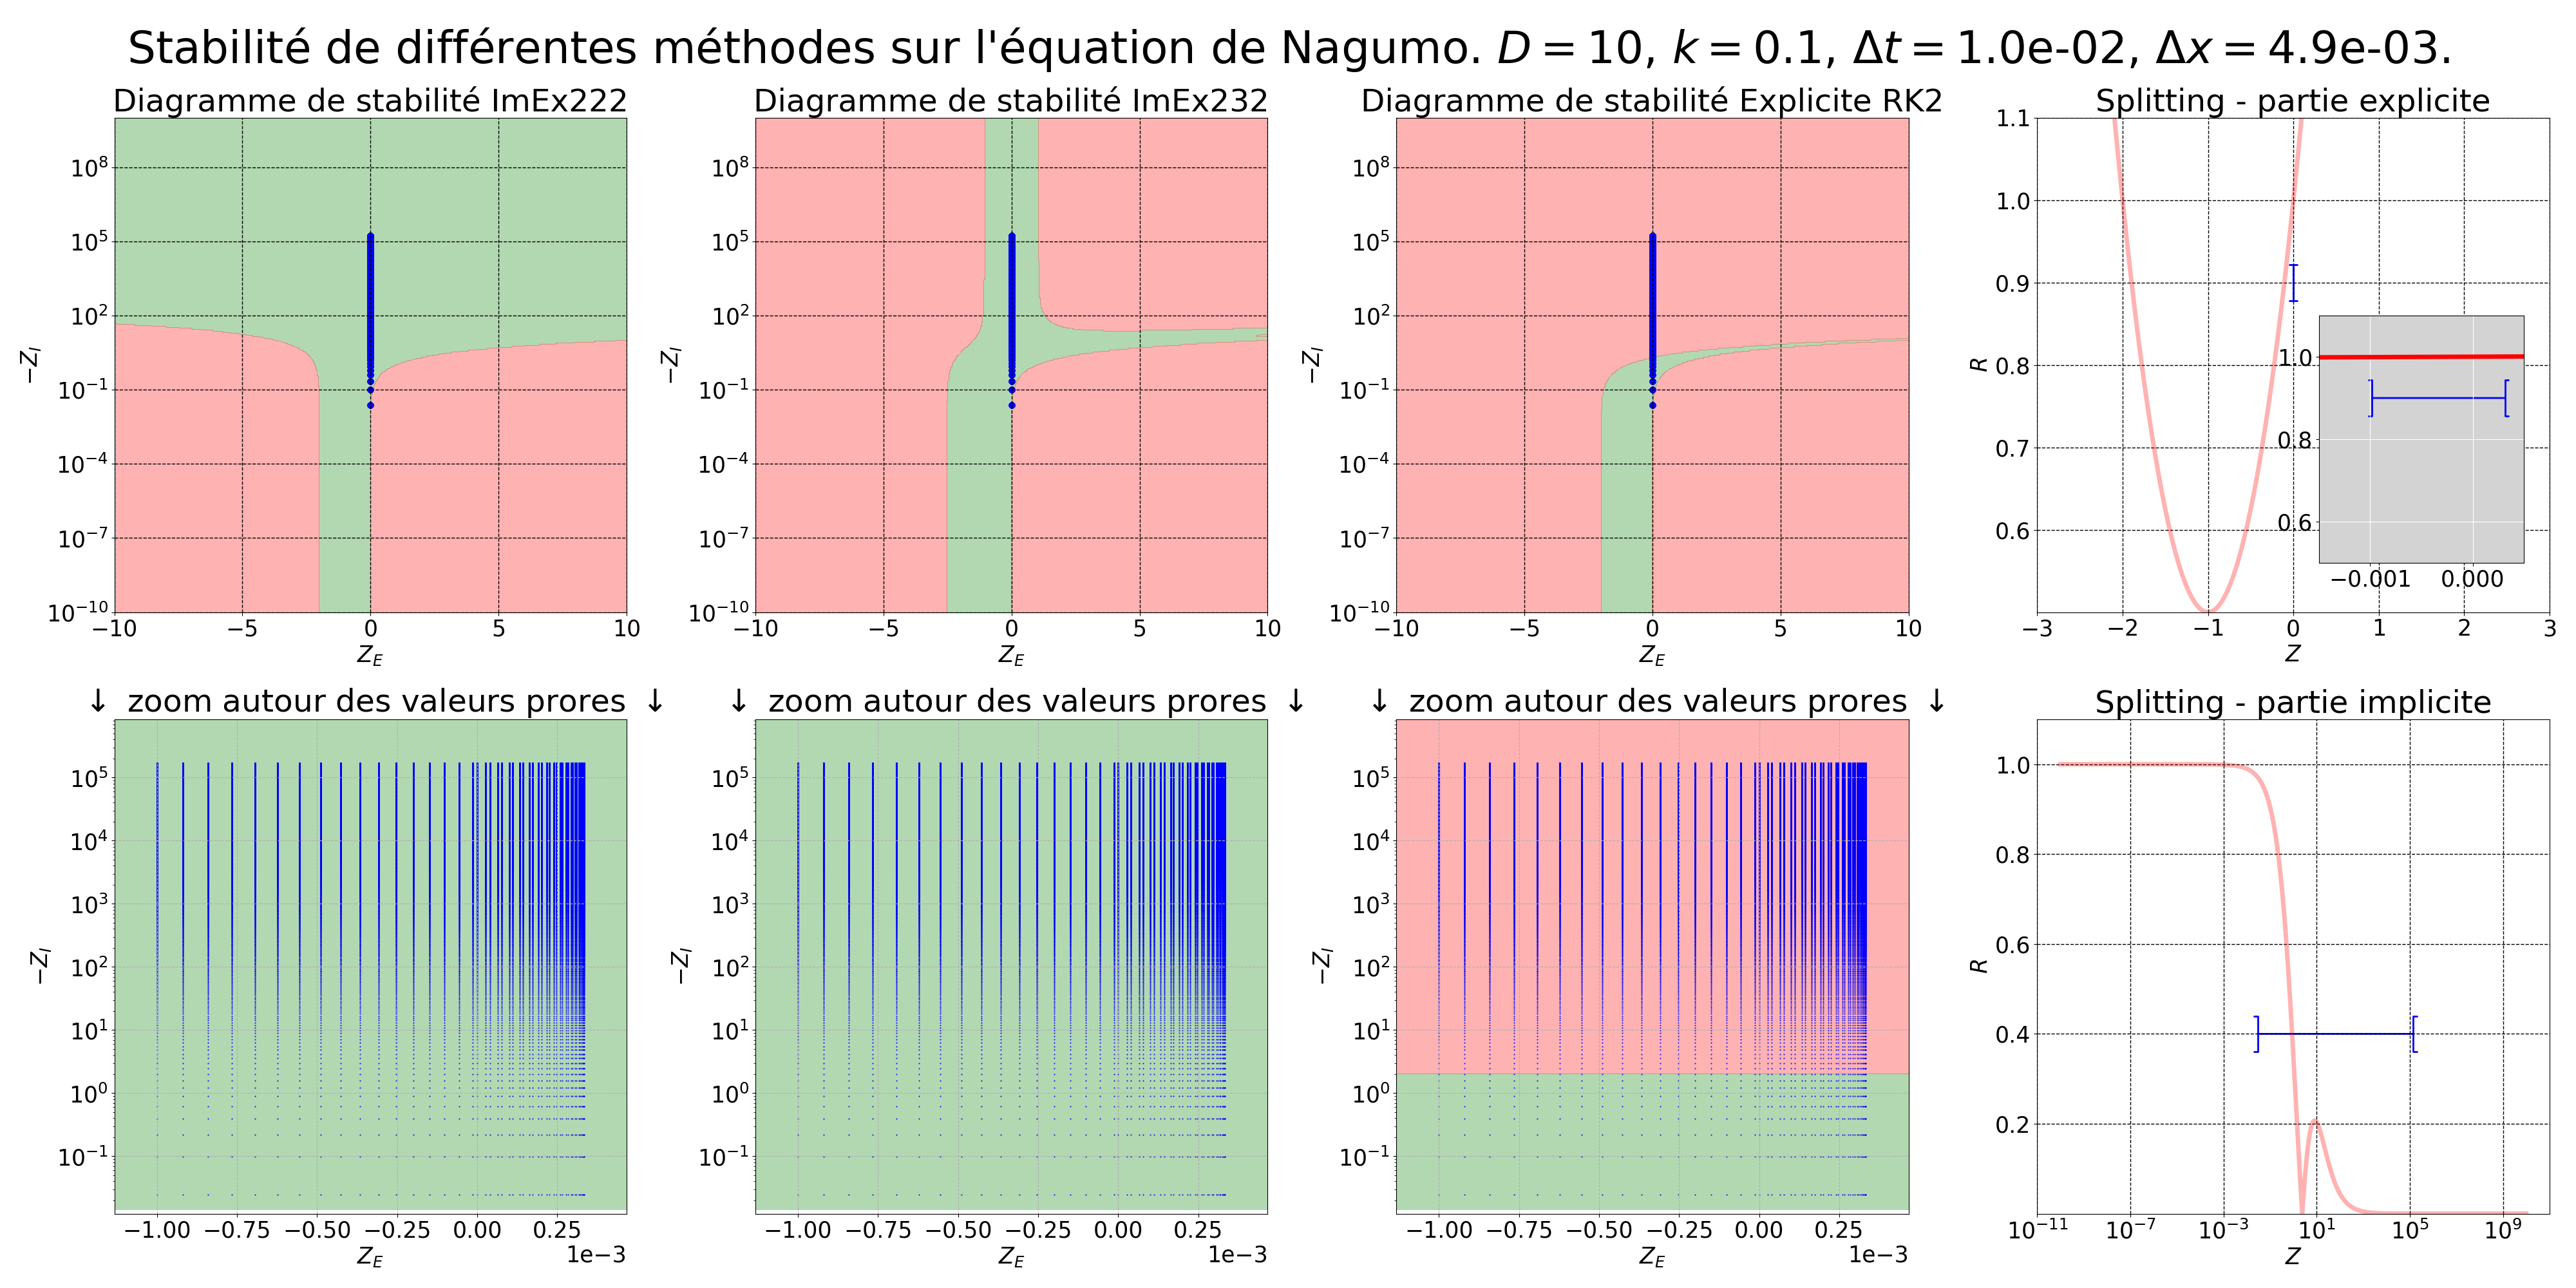
\includegraphics[width=0.8\textwidth]{media/4_travail/2_nagumo/stabilite/STABILITE_D10_k0.1_dt1.0e-02_dx4.9e-03.png}
            \caption{Cas diffusion plus raide, réaction moins raide\\D=10, k=0.1, dt=1.0e-02, dx=4.9e-03}
            \label{fig:stabilite_nagumo_b}
        \end{subfigure}

        \begin{subfigure}{\textwidth}
            \centering
            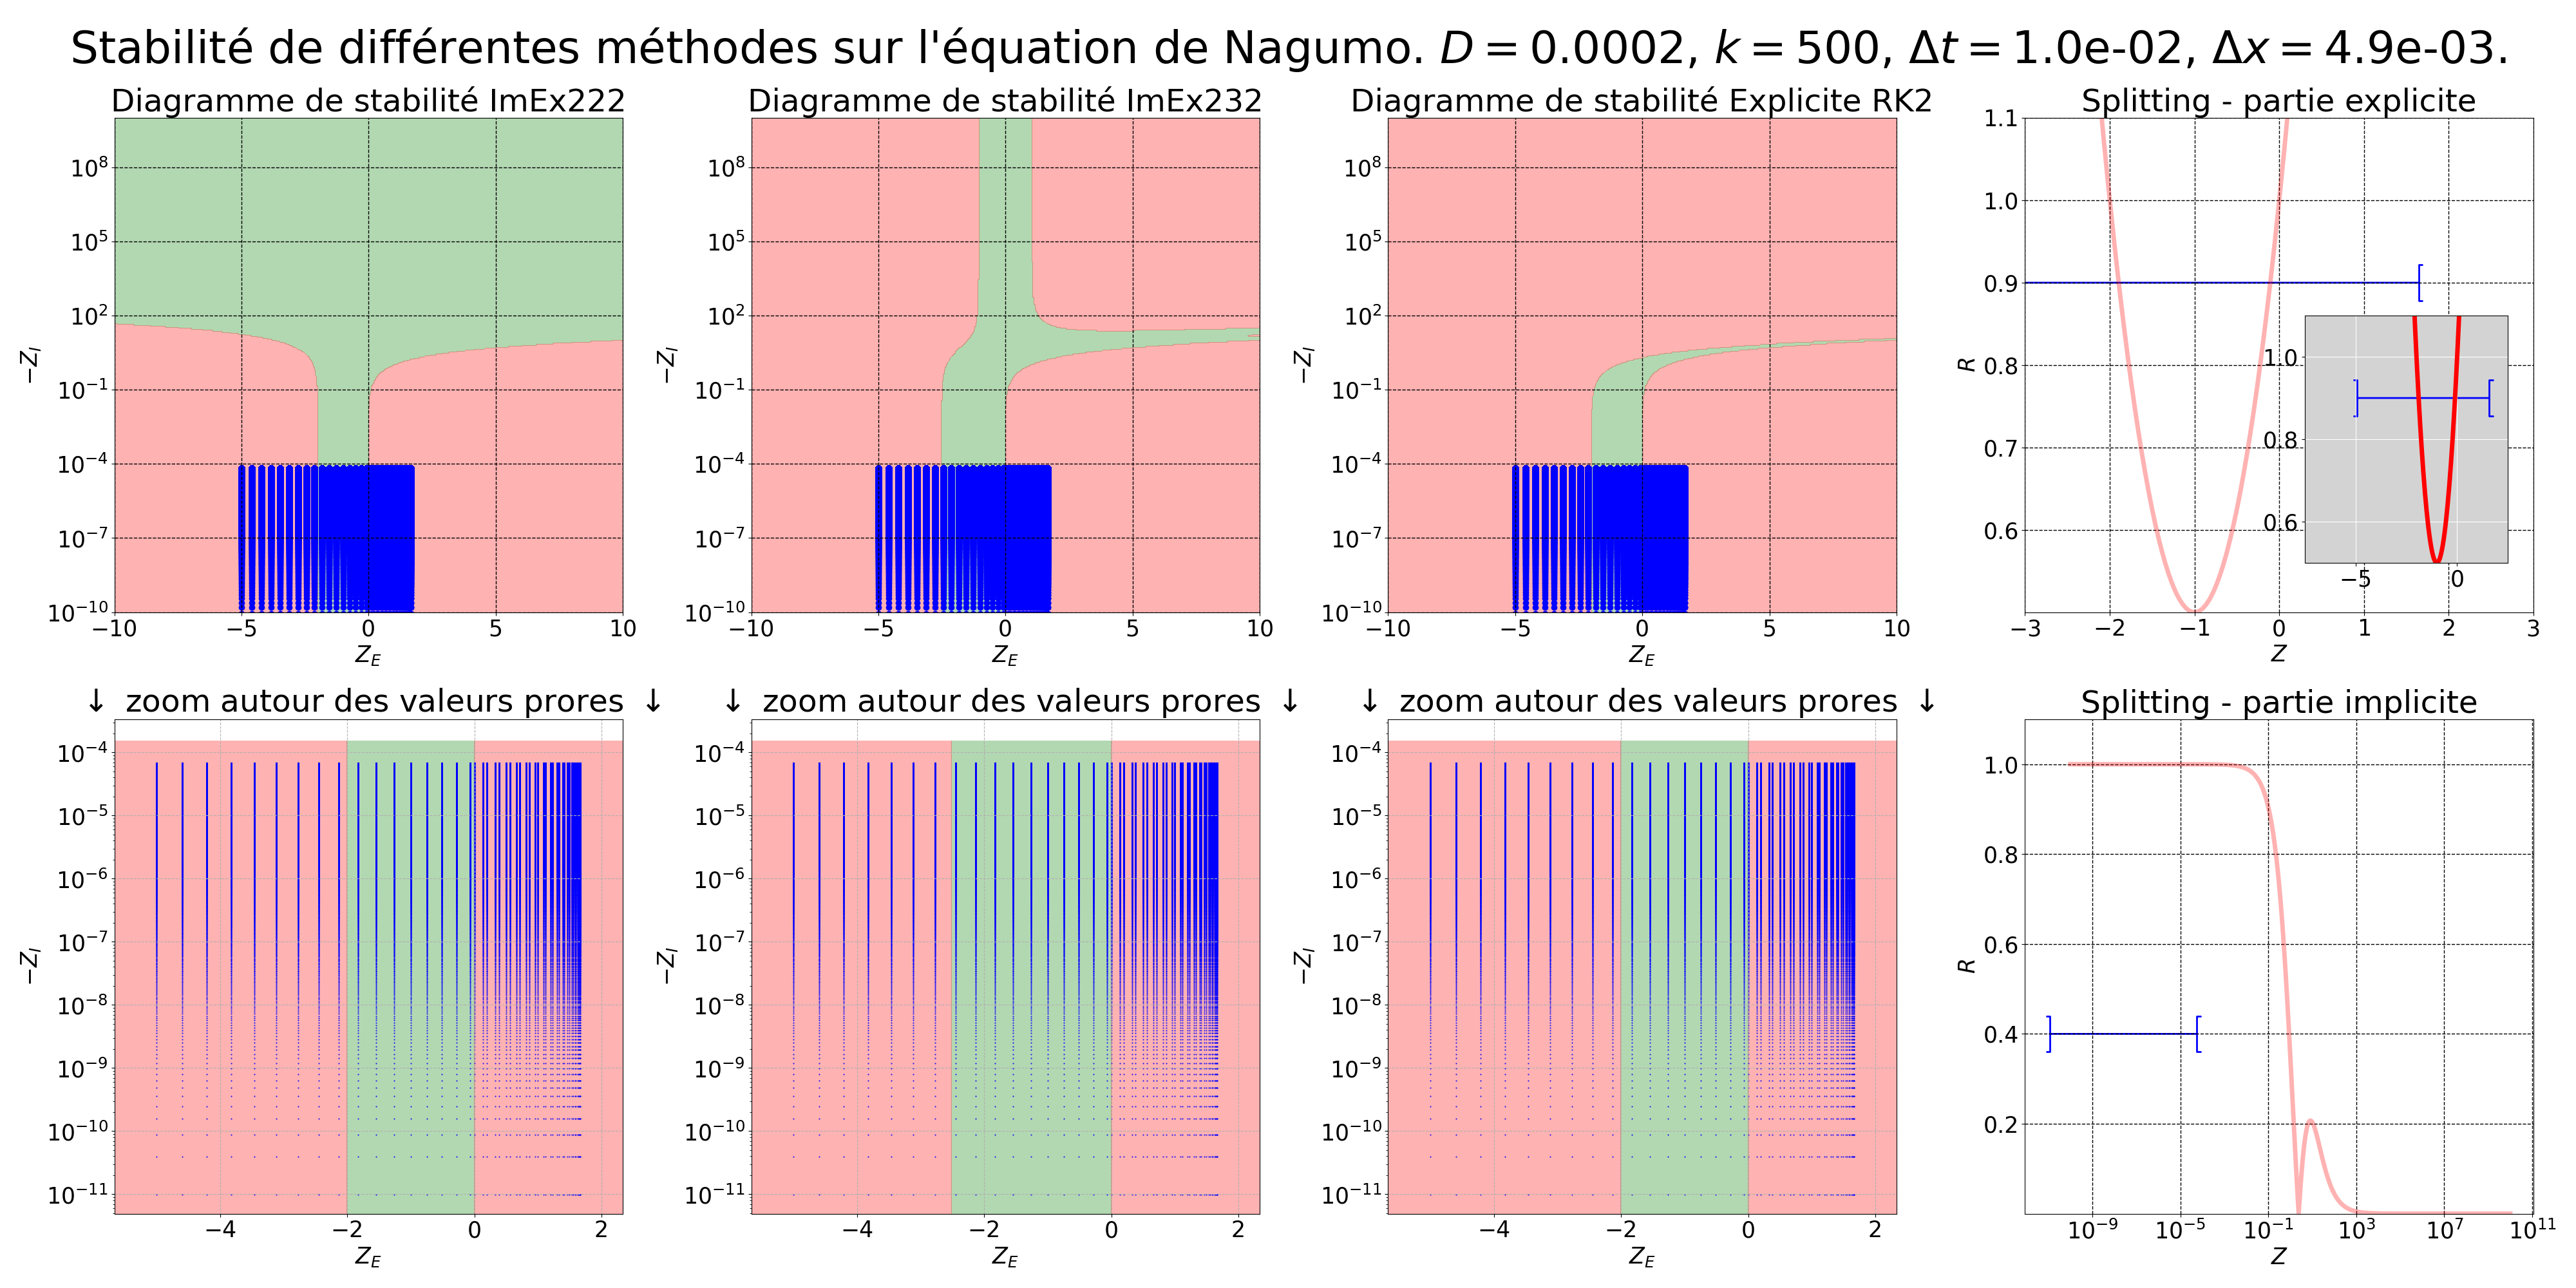
\includegraphics[width=0.8\textwidth]{media/4_travail/2_nagumo/stabilite/STABILITE_D0.0002_k500_dt1.0e-02_dx4.9e-03.png}
            \caption{Cas diffusion moins raide, réaction plus raide\\D=2e-4, k=500, dt=1.0e-02, dx=4.9e-03}
            \label{fig:stabilite_nagumo_c}
        \end{subfigure}
        
        \caption{Pour différents couples $D$ et $k$, diagrammes de stabilité des méthodes ImEx et de référence sur l'équation de Nagumo.}
        \label{fig:stabilite_nagumo}
    \end{figure}

        Le lecteur est invité à prendre un peu de temps pour comprendre la logique de ces graphiques car ils sont très éclairants. 
        Ces diagrammes permettent d'analyser respectivement la stabilité de la méthode ImEx222, de la méthode ImEx232, 
        ainsi qu'à titre de comparaison, la stabilité d'une méthode RKE d'ordre 2\footnote{Celle apparaissant dans ImEx222.} 
        et d'une méthode de splitting
        \footnote{Où l'on utilise les méthodes implicites et explicites de la méthode ImEx222 mais dans un contexte de splitting de Strang.}.
        Chaque colonne représente l'analyse d'une méthode différente.
        La première ligne présente le domaine de stabilité en fonction des indices spectraux $Z_E \in \mathbb{R}$ et $Z_I \in \mathbb{R}^-$. 
        Les points bleus représentent les couples d'indices spectraux intervenant dans la résolution de l'équation de Nagumo 
        pour les paramètres d'équation choisis ($D$ et $k$) et les paramètres de discrétisation retenus ($\Delta t$ et $\Delta x$). 
        La seconde ligne n'est qu'un zoom de la première autour de ces indices spectraux. 
        La dernière colonne (splitting) présente une disposition différente, puisque les opérateurs sont totalement découplés.
        La première ligne correspond à la fonction de stabilité de la méthode explicite (avec un zoom autour des indices spectraux de la réaction).
        la seconde ligne représente la fonction de stabilité de la méthode implicite. 
        Dans les deux cas, l'intervalle tracé en bleu représente la plage de valeurs d'indices spectraux balayés par chaque opérateur.

        \paragraph{Analyse}
            \subparagraph{Analyse générale}\label{par:analyse_generale_stab_nagumo}
                Analysons les domaines de stabilité des figures en \figref{fig:stabilite_nagumo}, pour l'instant nous ignorons les marqueurs bleus sur les figures.
                \begin{itemize}
                    \item[$\diamond$]\textbf{Méthode RKE2:} En troisième colonne, le diagramme de stabilité d'une méthode explicite naïve RKE2, sert de référence. 
                        Le domaine de stabilité accepte des valeurs propres négatives de magnitude deux, ce qui est résultat classique des méthodes Runge et Kutta explicites d'ordre deux.
                        Ainsi domaine de stabilité s'étend jusqu'à $-2$ selon l'axe portant $Z_E$ tant que la valeur propre $Z_I$ est négligeable.
                        De même le domaine de stabilité s'étend jusqu'à $-2$ selon $Z_I$ tant que la valeur propres $Z_E$ est négligeable. 
                        Enfin il y a une zone intermédiaire quand $Z_E$ et $Z_I$ sont tous les deux de l'ordre de l'unité\footnote{Attention à l'échelle logarithmique.},
                        où la raideur résultante est $Z_E+Z_I$.

                    \item[$\diamond$]\textbf{Méthode ImEx232:} En observant la seconde colonne, nous constatons que la méthode ImEx232 maintient un domaine de stabilité restreint (jusqu'à $-2$) selon l'axe $Z_E$,
                        mais selon l'axe $Z_I$, le domaine de stabilité s'est étendu considérablement. C'est logique puisque la valeurs propre $Z_E$ est explicitée,
                        sont domaine pris seul n'a évolué, et la valeur propre $Z_I$ peut être très raide (très négative) puisque la méthode explicite l'opérateur lié à $Z_I$.
                        % Voir que le domaine de stabilité est légèrement décalé vers la droite quand $Z_I$ est grand

                    \item[$\diamond$]\textbf{Méthode ImEx222:} Passant à la première colonne, le domaine de stabilité ImEx222 resemble beaucoup à celui de l'ImEx232. Seulement, le domaine de stabilité s'élargit considérablement
                        selon $Z_E$, pourvus que $Z_I$ soit assez grand. Cette propriété est remarquable, cela signifie que la méthode traite couple les raideurs dans sont traitement. 
                        Plus précisément, plus l'opérateur implicité est raide, plus l'opérateur explicité peut être raide\footnote{Cette analyse est partiellement erronée, nous verrons 
                        pourquoi au prochain paragraphe.}.
                        % AFAIRE :
                        % Pourquoi ? Qu'est ce qui change fondamentalement ? 
                        % ---> certaines VP positives ont une fonction d'amplification négatives pour la réaction, ca pourrait poser problème (perte d'ordre ?)
                        % justement pour le splitting c'est pas le cas, et lui il ne perd pas l'ordre ??? ... 
                \end{itemize}
            \subparagraph{Analyse selon les paramètres de l'équation $k$ et $D$}
                Analysons grace au graphiques \figref{fig:stabilite_nagumo} la disposition des valeurs couples de valeurs 
                propres mis en jeu par l'équation de Nagumo selon les paramètre $k$ et $D$. Les paramètres de simulation: $\Delta t$ et $\Delta x$ sont fixés.
                Les jeux de valeurs choisis sont $(k,D)=(1,1)$, $(k,D)=(0.1,10)$, $(k,D)=(500,2\, 10^{-4})$. 
                Le produit $kD$ est maintenu égal à un, ainsi la vitesse de propagation est toujours la même.
                Ces couples de valeurs propres $Z_E,Z_I$ mis en jeu par les opérateur de l'équation sont tracés en bleus
                \footnote{Pour les $Z_I$ le spectre est discret, pour $Z_E$, le spectre est continu, il a donc fallut échantillonnés le long de l'axe $Z_E$}.
                %---> AFAIRE : au lieu d'un scatter de faire un plot pour représenter la continuité du spectre de l'opérateur de réaction.
                \begin{itemize}
                    \item[$\diamond$]\textbf{Cas standard, $(k,D)=(1,1)$} - \figref{fig:stabilite_nagumo_a}:\\
                        Dans ce cas, la raideur de la diffusion ($Z_I$) déstabilise la méthode RKE2 (on voit que de nombreux couples de v.p. entrent dans le zones rouges quand $Z_I$ augmente).
                        Pour ces valeurs de $(\Delta x, \Delta t)$ cette méthode n'est donc pas viable.
                        C'est tout à fait normal, les méthodes imposent des pas de temps très restrictifs sur les problèmes de diffusion.
                        En revanche, les méthodes ImEx sont tout à fait stable puisque, comme constaté précédemment, le domaine de stabilité s'étend infiniment quand $Z_I \rightarrow -\infty$.
                        Le point notable est que certains couples de valeurs propres tombent malgré tout dans une zone instable (en bas à gauche). Mais cela n'est pas un problème car il s'agit 
                        de couples de valeurs propres ou la valeur propres
                        \footnote{Dans cette section, nous identifions valeurs propres $\lambda$ et indices spectraux $z = \lambda \Delta t$ puisque le pas de temps $\Delta t$ est maintenu constant. Cette identification permet de discuter directement en termes de raideur des opérateurs.}
                        de l'opérateur de réaction ($Z_E$) est positive. Donc la méthode n'est pas instable au sens ou elle reflète simplement
                        la dynamique explosive de la réaction. D'ailleurs si en se penchant sur le graphique de la partie explicite du splitting, on constante qu'il y a une zone 
                        (correspondant à $Z_E$ positive) ou la fonction d'amplification est d'amplitude supérieure à un, le splitting reproduit donc fidèlement la dynamique de la réaction.
                        Ce qui peut être un problème est l'inverse, 
                        pour les méthodes ImEx, il y a des couples de valeurs propres où $Z_E$ est positif et où la fonction d'amplification est d'amplitude inférieure à un. 
                        Cela pourrait être un frein pour reproduire fidèlement la dynamique explosive de la réaction dans les zones concernées
                        \footnote{Il n'est pas évident d'avoir \textit{a priori} la bonne intuition car peut être que la diffusion calme en quelque sorte 
                        le caractère explosif de la réaction et qu'alors une fonction d'amplification d'amplitude $< 1$ est normal... Restons prudent sur cette analyse.}.
                    \item[$\diamond$]\textbf{Cas diffusion raide, réaction peu raide, $(k,D)=(0.1,10)$}  - \figref{fig:stabilite_nagumo_b}:\\
                        Ici, $D=10$ donc toutes les valeurs propres liées à la diffusion sont multipliées par 10 par rapport au cas précédent. 
                        De fait la méthode RK2E de référence présente des instabilités pour encore plus de couples de valeurs propres est n'est pas pas viable.
                        Concernant les méthodes ImEx222 et ImEx232 elles sont stables, et cette fois-ci toutes les valeurs propres liées à la 
                        dynamique explosive de la réaction sont amorties. 
                        % ---> AFAIRE voir expérimentalement ce que ça donne... 
                    \item[$\diamond$]\textbf{Cas diffusion peu raide, réaction très raide$(k,D)=(500,2\, 10^{-4})$} - \figref{fig:stabilite_nagumo_c}\\
                        Dans ce cas de figure, $k=500$. La grande valeur du coefficient de réaction rend cette dernière très raide. 
                        Cela à pour effet de dilater selon l'axe des abscisse les indices spectraux puisque $Z_E \in [- 500 \Delta t, + 1000 \Delta t]$
                        alors que dans le cas $k=1$: $Z_E \in [- \Delta t , 2\Delta t]$.
                        Ici la méthode méthode explicite au sein des ImEx n'est plus stable pour la réaction, ainsi toutes les méthodes deviennent instables. 
                        Le splitting également devient instable car il utilise aussi la méthode RK2E pour la réaction. 
                        Le fait que la méthode explicite de l'ImEx soit instable pour l'opérateur explicité peu sembler un obstacle infranchissable,
                        cependant ce n'est pas si simple.
                        Pour illustrer ce point, étendons l'analyse avec le cas spécial en \figref{fig:stabilite_nagumo_cas_special}, dans ce cas la réaction est toujours raide $k=500$ mais la diffusion est également très raide car $D=500$
                        \footnote{Jusqu'ici, la vitesse de propagation était la même dans tous les scénarios puisque $kD$ était maintenu constant. Dans le scénario présenté ici, ce n'est plus le cas}
                        Alors la méthode ImEx222 devient stable, comme vu en \ref{par:analyse_generale_stab_nagumo}, plus l'opérateur traité implicitement est raide, 
                        plus la méthode permet à l'opérateur traité explicitement d'être raide. C'est un cas remarquable ou le couplage intervenant au sein de la méthode ImEx
                        la rend plus stable que le splitting !
                \end{itemize}
                \begin{figure}[htbp]
                    \centering
                    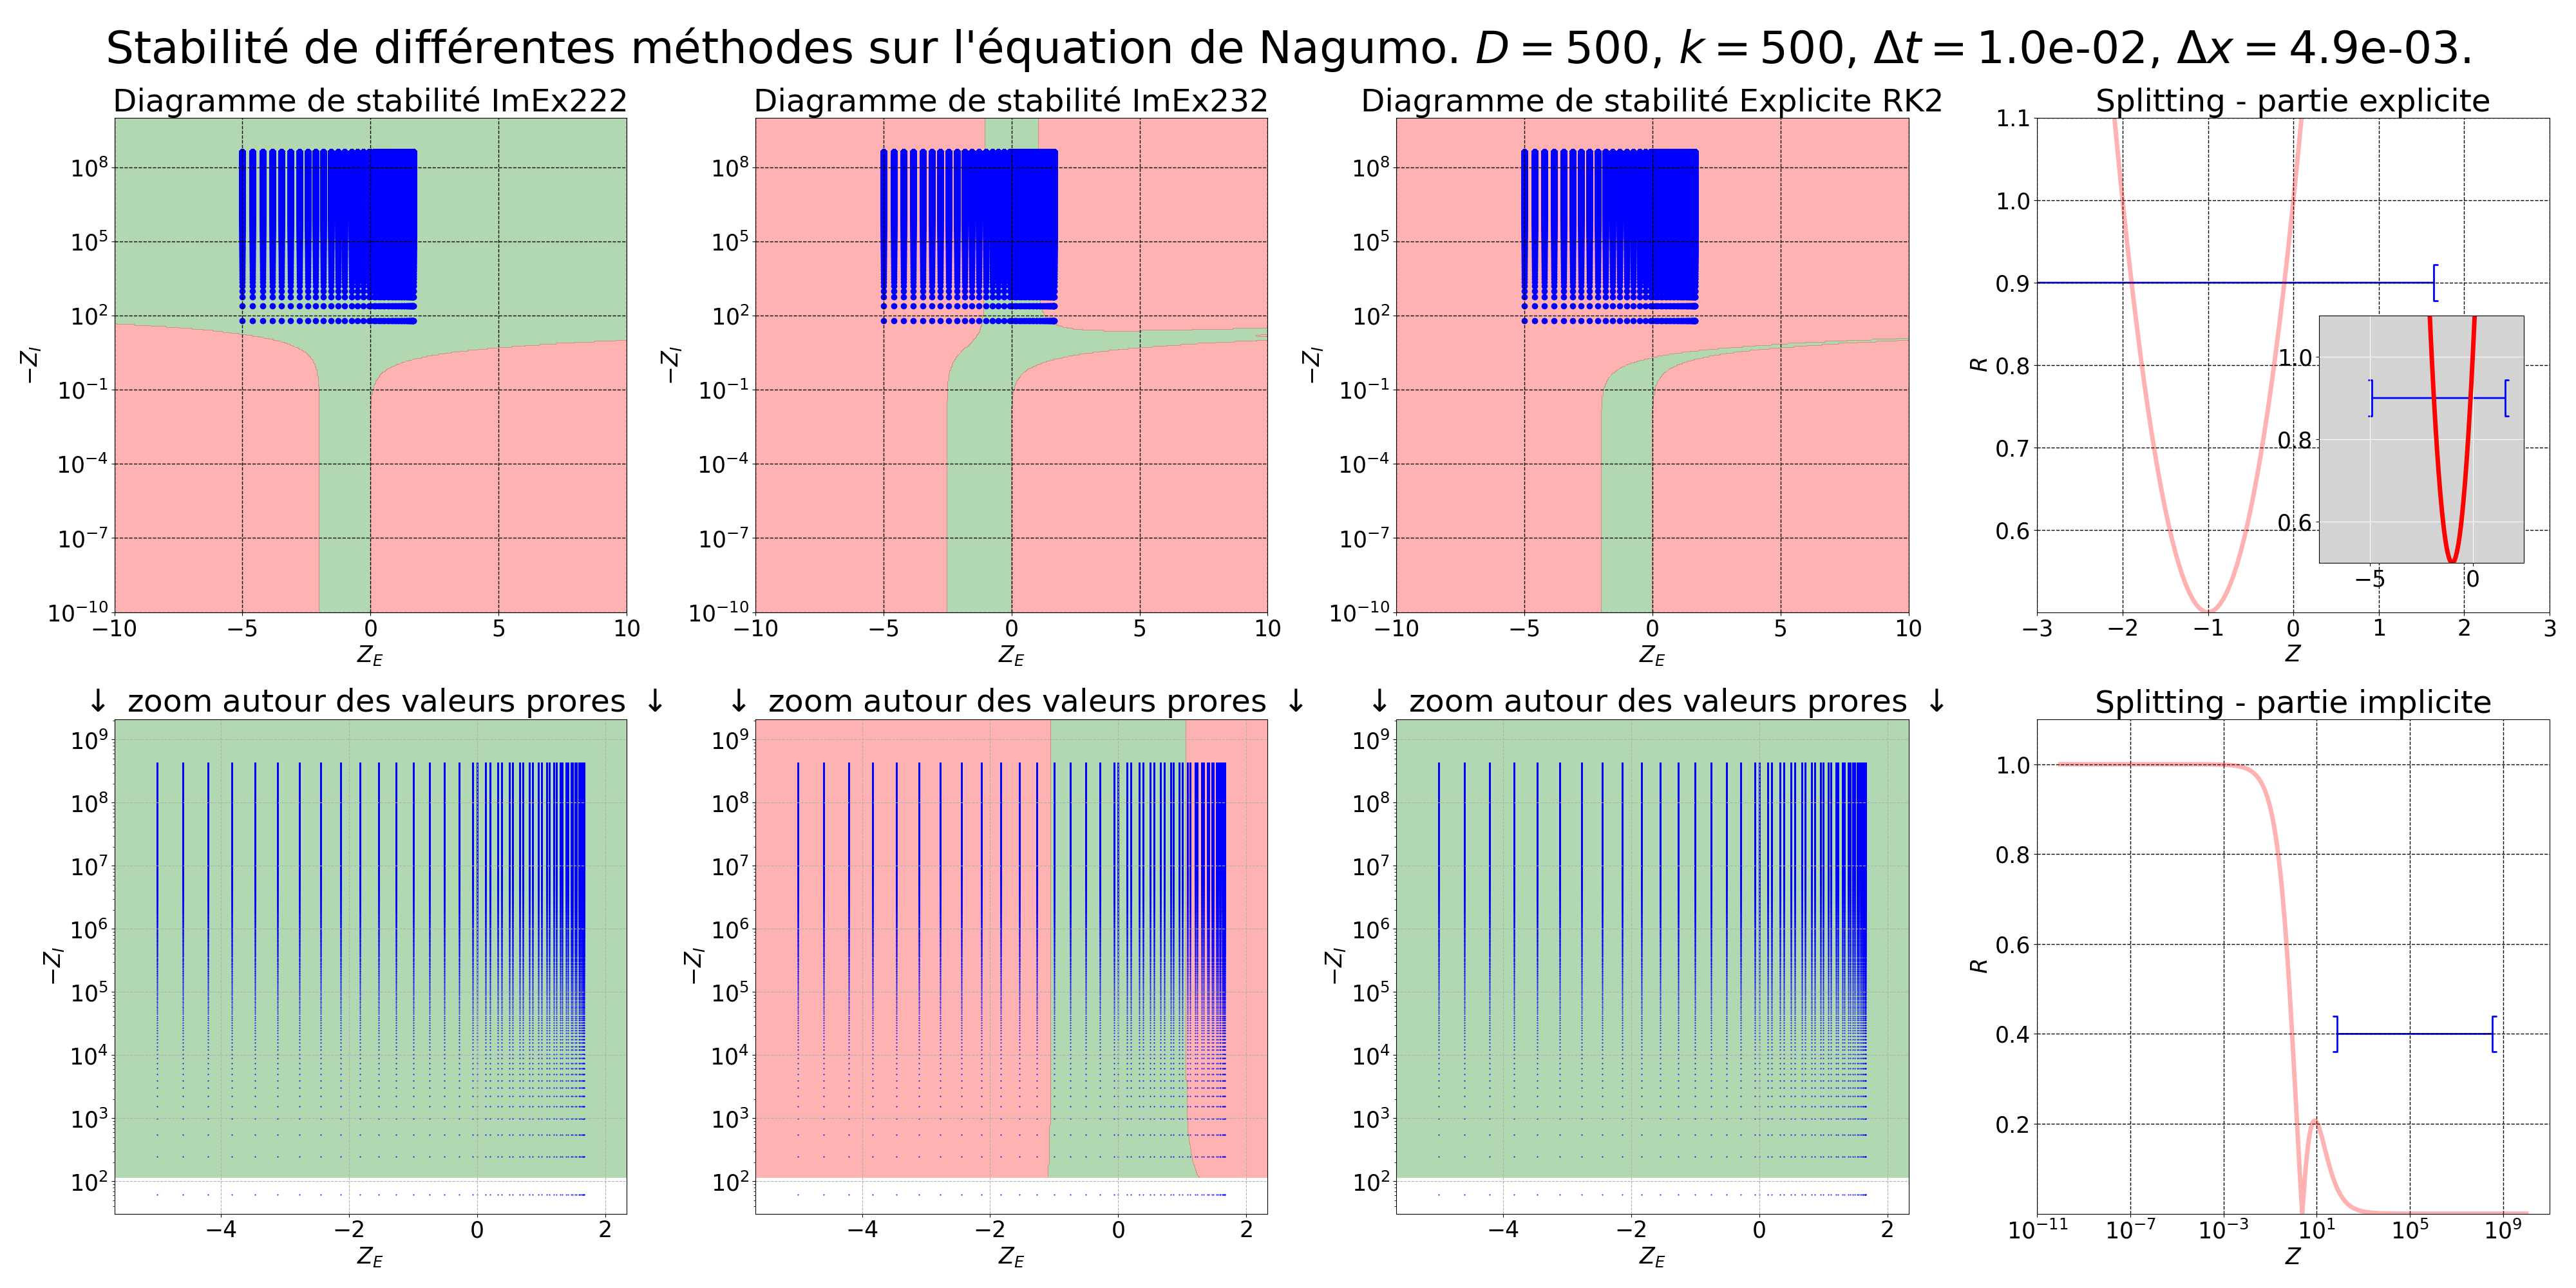
\includegraphics[width=0.8\textwidth]{media/4_travail/2_nagumo/stabilite/STABILITE_D500_k500_dt1.0e-02_dx4.9e-03.png}
                    \caption{Pour $k=500$ et $D=500$: diagrammes de stabilité des méthodes ImEx et de référence sur l'équation de Nagumo.}
                    \label{fig:stabilite_nagumo_cas_special}
                \end{figure}
            \subparagraph{Analyse selon les paramètres de simulation $\Delta t$ et $\Delta x$}
                